\documentclass[aps,twocolumn,prd,superscriptaddress,nofootinbib,floatfix]{revtex4-2}



%%%%%%%%%%%%% Packages %%%%%%%%%%%%%

% general
%\usepackage[utf8]{inputenc}
\usepackage{titlesec}

  
% math
\usepackage{mathtools}
\usepackage{amsfonts}
\usepackage{amssymb}
\usepackage{mathrsfs}
\usepackage{bbm}
\usepackage{slashed}
\usepackage{amsmath}
\usepackage{bm}
\usepackage{bbold}


% graphics and colors
\usepackage{graphicx}
\usepackage{color}
\usepackage{colortbl}
\usepackage{array}

% floats
\usepackage{float}
\usepackage{placeins}
\usepackage{booktabs}
%\usepackage{caption}
\usepackage[caption=false]{subfig}
\captionsetup{justification=centerlast}
\usepackage{makecell}
\usepackage{tabstackengine}


% units and refs
\usepackage{xspace}
\usepackage{hyperref}
\usepackage[nameinlink]{cleveref}
\usepackage{bookmark}
\usepackage{siunitx}


% Other
\usepackage{xifthen}
\usepackage{xcolor}
\hypersetup{
	colorlinks,
	linkcolor={red!75!black},
	citecolor={blue!75!black},
	urlcolor={blue!75!black}
}

\usepackage[utf8]{inputenc}
\allowdisplaybreaks[4]


%%%%%%%%%%%%%%%%%%%%%%%%%%%%%%%%%%%%%%%%

%--- start of the macros paper%
\newcommand{\hlambda}{\hat{\lambda}}
\newcommand{\LQCD}{\Lambda_{\text{\tiny QCD}}}
\newcommand{\eb}{\epsilon_{{b}}}
\newcommand{\muq}{\mu_{\textrm{q}}}
\newcommand{\mud}{\mu_{\textrm{d}}}
\newcommand{\mub}{\mu_{{b}}}
\newcommand{\mubo}{\bar{\mu}_{{b}}}
\newcommand{\mudo}{\bar{\mu}_{\textrm{d}}}
\newcommand{\muqo}{\bar{\mu}_{\textrm{q}}}
\newcommand{\MN}{M_{\textrm{N}}}
\newcommand{\mq}{m_{\textrm{q}}}
%\renewcommand{\md}{m_{\text{d}}}
\newcommand{\Md}{M_{\text{d}}}
\newcommand{\Mq}{M_{\text{q}}}
\newcommand{\Mb}{M_{{b}}}
\newcommand{\Mqb}{M_{\text{q}/{b}}}
\newcommand{\energyq}{\varepsilon_{\text{q}}}
\newcommand{\Lag}{\mathcal{L}}
\newcommand{\ua}{\mathrm{U(1)_A}}
\newcommand{\diag}{\mathrm{diag}}
\newcommand{\MeV}{\;\text{MeV}}
\newcommand{\GeV}{\;\text{GeV}}
\newcommand{\fm}{\;\text{fm}}
\newcommand{\rmi}{\mathrm{i}}
\newcommand{\rmd}{\mathrm{d}}
\newcommand{\rme}{\mathrm{e}}
\newcommand{\Nc}{N_{\mathrm{c}}}
\newcommand{\Nf}{N_{\mathrm{f}}}
\newcommand{\Tc}{T_{\mathrm{c}}}
\newcommand{\bB}{\boldsymbol{B}}
\newcommand{\bE}{\boldsymbol{E}}
\newcommand{\bgamma}{\vec{\gamma}}
\newcommand{\tr}{\text{tr}}
\newcommand{\Tr}{{\text{Tr}}}
\newcommand{\bp}{\vec{p}}
\newcommand{\Phifund}{\Phi_{\text{\tiny{fund}}}}
\newcommand{\rhos}{\rho_{\rm \phi}}
\newcommand{\rhod}{\rho_{\rm d}}
\newcommand{\Zq}{Z_{q}}
\newcommand{\Zphi}{Z_{\phi}}
\newcommand{\Zd}{Z_{d}}
\newcommand{\ZV}{Z_{V}}
\newcommand{\Zo}{Z_{\omega}}
\newcommand{\Zb}{Z_{b}}
\newcommand{\lambdas}{\lambda_{q\phi}}
\newcommand{\lambdad}{\lambda_{qd}}
\newcommand{\lambdasd}{\lambda_{q \phi/ d}}
\newcommand{\lambdaV}{\lambda_{qV}}
\newcommand{\lambdao}{\lambda_{q\omega}}
\newcommand{\lambdab}{\lambda_{qb}}
\newcommand{\lambdabd}{\lambda_{qdb}}
\newcommand{\lambdabo}{\lambda_{b\omega}}

\newcommand{\hs}{h_{q\phi}}
\newcommand{\hd}{h_{qd}}
\newcommand{\hV}{h_{qV}}
\newcommand{\ho}{h_{q\omega}}
\newcommand{\hsd}{h_{q \phi/d}}
\newcommand{\hsb}{h_{q/b \phi}}
\newcommand{\hb}{h_{b\phi}}
\newcommand{\hbo}{h_{\omega \rm b}}
\newcommand{\hdo}{h_{\omega \rm d}}
\newcommand{\hqo}{h_{\omega \rm q}}
\newcommand{\hqdb}{h_{qdb}}
\newcommand{\hqb}{h_{qb}}
\newcommand{\dynA}{D}
\newcommand{\dynB}{D}
\newcommand{\bolda}{\boldsymbol{a}}
\newcommand{\boldabar}{\bar{\boldsymbol{a}}}
\newcommand{\feyn}[1]{
	\setbox0=\hbox{\ensuremath{#1}}
	\hbox to\wd0{\hbox to0pt{\hbox to\wd0{\hss/\hss}\hss}\box0}}

\newcommand{\nsat}{n_{b}^{\text{(sat)}}}
\newcommand{\Vb}{V_{b}}
\newcommand{\nb}{n_{b}}

%--- end of the definition of KF ---%
%%%%%%% Dirac slashes %%%%%%
\def\pslash{p\hspace{.015cm}\llap{/}\hspace{.015cm}}
\def\pa{\partial}
\def\al{\alpha}
\def\pr{\prime}
\def\dr{{D\!\llap{/}}\,}
\def\Dr{{D\llap{/}}\,}
% \def\k{k\llap{/}}
\def\ip{p\llap{/}}
\def\iq{q\llap{/}}
\def\ik{k\llap{/}}
\def\il{l\llap{/}}
\def\ir{r\llap{/}}
\def\es{\epsilon\llap{/}}
\def\A{A\!\llap{/}}
%%%%%%%%%%%% refs %%%%%%%%%%%%%%%%%%%
\def\sectionautorefname{Sec.\!}
\def\figureautorefname{Fig.\!}
\def\tableautorefname{Tab.\!}

%%%%%%%%%%%%% Options %%%%%%%%%%%%%
\setkeys{Gin}{width=0.48\textwidth}
\captionsetup{justification=centerlast}
\sisetup{range-units=single}

%\newcommand{\tr}{{\text{tr}}}

\newcommand*{\eg}{e.g.\@\xspace}
\newcommand*{\ie}{i.e.\@\xspace}
\newcommand*{\etc}{etc.\@\xspace}
\newcommand*{\cf}{cf.\@\xspace}


%%%%%%%%%%%%% Math commands %%%%%%%%%%%%%
% symbols
\newcommand{\sumint}{\int\hspace{-4.8mm}\sum}
\newcommand{\imag}{\text{i}}
\newcommand{\pz}{$P_z$}

\newcommand{\tinytext}[1]{\text{\tiny{#1}}}

%%%%%%%%%%%%% Graphic paths %%%%%%%%%%%%%
\graphicspath{{./figures/}}


%%%%%%%%%%%%%% for corrections %%%%%%%%%%%
\newcommand{\coljh}[1]{\textcolor{blue}{#1}}
\newcommand{\colwj}[1]{\textcolor{red}{#1}}
\newcommand{\colsy}[1]{\textcolor{green}{#1}}
\newcommand{\colcj}[1]{\textcolor{cyan}{#1}}

\newcommand{\gettitle}{}

% affiliations
\newcommand{\getFudanAffiliation}{\affiliation{Key Laboratory of Nuclear Physics and Ion-beam Application (MOE),
and Institute of Modern Physics, Fudan University, Shanghai 200433, P.R. China}}

\newcommand{\getNSFCFudanAffiliation}{\affiliation{Shanghai Research Center for Theoretical Nuclear Physics, NSFC and Fudan University, Shanghai 200438, P.R. China}}

\newcommand{\getDalianAffiliation}{\affiliation{School of Physics, Dalian University of Technology, Dalian, 116024, P.R. China}}

\newcommand{\getGiessenAffiliation}{\affiliation{Institut f\"ur Theoretische Physik, Justus-Liebig-Universit\"at Gie\ss en, 35392 Gie\ss en, Germany}}


\hypersetup{
	colorlinks,
	linkcolor={red!75!black},
	citecolor={blue!75!black},
	urlcolor={blue!75!black},
	%%%%%%%%%%%%%%%%%%%%%%%%%%%%%%%%%%
	pdftitle={\gettitle},
	pdfauthor={Zelle},
	pdfkeywords={effective theory} {analytic continuation}
	{correlations functions} {hadronization}
	{functional renormalisation group}
	{real time} {bound states}
	bookmarksopen=true,
	bookmarksopenlevel=2,
	bookmarksnumbered=true
}


\begin{document}


%%%%%%%%%%%%%%%%%%%%%%%%%%%%%%%%%%%%%%%%%%%%%
\newpage

%\appendix 
\renewcommand{\thesubsection}{{S.\arabic{subsection}}}
\setcounter{section}{0}
\titleformat*{\section}{\centering \Large \bfseries}

\onecolumngrid

	

%\begin{widetext}
%	\newcounter{totalequations}
\section*{Supplemental Materials}
%	\parttoc % Insert the appendix TOC
The supplemental materials provide some details of the 2+1 flavor low energy effective field theory within the functional renormalization group approach, \Cref{app:LEFT2p1}, preliminary results of temperature fluctuations calculated in QCD within fRG, \Cref{app:cn-QCD}, hyper-order fluctuations of temperature, \Cref{app:hyper-order}, ratios of temperature fluctuation cumulants, \Cref{app:cn-ratios}, relation between the temperature $T$ and the mean transverse momentum $\langle p_{T} \rangle$, \Cref{app:T-pT-relation}.
%%%%%%%%%%%%%%%%%%%%%%%%%%%%%%%%%%%%%%%%%%%%%%%%%%%%%%%%%%%%


%%%%%%%%%%%%%%%%%%%%%%%%%%%%%%%%%%%%
\subsection{2+1 flavor low energy effective field theory within the fRG}
\label{app:LEFT2p1}

In this appendix, we recapitulate the setup of the 2+1 flavor low energy effective field theory (LEFT) within the functional renormalization group used in this work. More details about the 2+1 LEFT can be found in \cite{Wen:2018nkn}. The effective action reads
\begin{align}
    \Gamma_{k}[\Phi]=&\int_x \bigg\{ \bar{q} \big[\gamma_\mu \partial_\mu-\gamma_0(\mu+igA_0)\big]q+h_k\,\bar{q} \,\Sigma_5 q+\text{tr}\big(\partial_\mu \Sigma \cdot \partial_\mu\Sigma^\dagger \big)+V_{\mathrm{\tiny{matt}},k}(\phi)+V_{\mathrm{\tiny{glue}}}(L, \bar L)\bigg\}\,,\label{eq:action}
\end{align}
with the shorthand notation $\int_{x}=\int_0^{\beta}d x_0 \int d^3 x$ and $\beta=1/T$, where $T$ stands for the temperature. The subscript $k$ in $\Gamma_{k}$ indicates that an infrared (IR) cutoff is applied to the effective action, such that quantum and thermal fluctuations of momenta $p\lesssim k$ are suppressed. The full effective action is resolved as $k \to 0$, and thus $k$ plays a role as the renormalization group (RG) scale. The field $\Phi=(q, \bar q, \phi)$ includes the three-flavor quark field $q=(q_u, q_d, q_s)^\intercal$ and the scalar and pseudoscalar meson fields $\phi=(\sigma, \pi)$. The mesons are in the adjoint representation of the $\mathrm{U}(N_f=3)$ group, which reads
\begin{align}
    \Sigma=T^a(\sigma^a+i \pi^a)\,, \quad a=0,\,1,...,8\,,\label{}
\end{align}
with
\begin{align}
    T^{0}=\frac{1}{\sqrt{2N_{f}}}\mathbb{1}_{N_{f}\times N_{f}}\,,\label{}
\end{align}
and
\begin{align}
    T^a=\frac{\lambda^a}{2} \quad(a=1,...,8)\,, \label{}
\end{align}
where $\lambda^a$ are the Gell-Mann matrices. The quark and meson fields interact with each other through the Yukawa coupling $h_k$ with
\begin{align}
    \Sigma_5=T^a(\sigma^a+i \gamma_5\pi^a)\,.\label{}
\end{align}
The quark chemical potential $\mu$ in \labelcref{eq:action} is related to the baryon chemical potential $\mu_B$ with $\mu=\mu_B/3$, where other chemical potentials, e.g., the chemical potentials for the electric charge and strangeness, are assumed to be vanishing.

%
%%%%%%%%%%%%%%%%%%%%%%%%%%%%%
\begin{figure}[t]
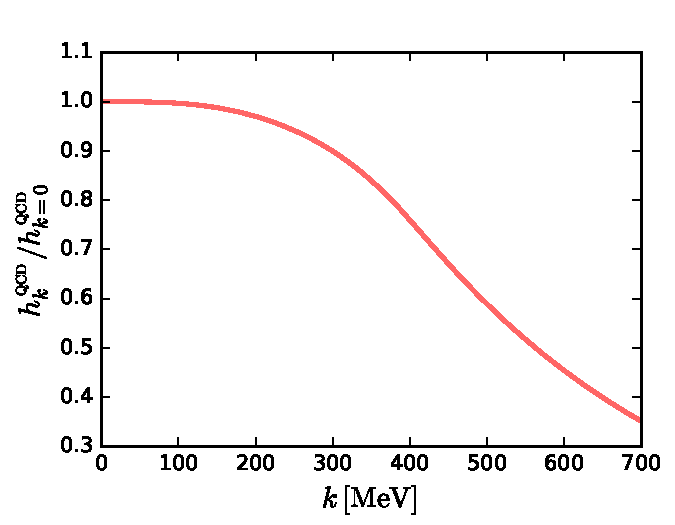
\includegraphics[width=0.45\textwidth]{hQCD-k}
\caption{Yukawa coupling, normalized to unity for $k=0$, as a function of the RG scale $k$, computed from the first-principles QCD within the fRG in the vacuum \cite{Fu:2019hdw}.}
\label{fig:hQCD-k}
\end{figure}
%%%%%%%%%%%%%%%%%%%%%%%%%%%%%
%

%
%%%%%%%%%%%%%%%%%%%%%%%%%%%%%
\begin{figure*}[t]
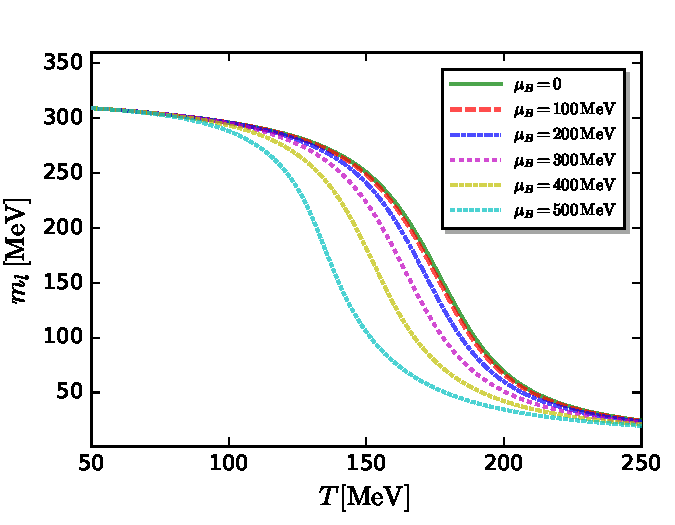
\includegraphics[width=0.45\textwidth]{ml}\hspace{0.5cm}
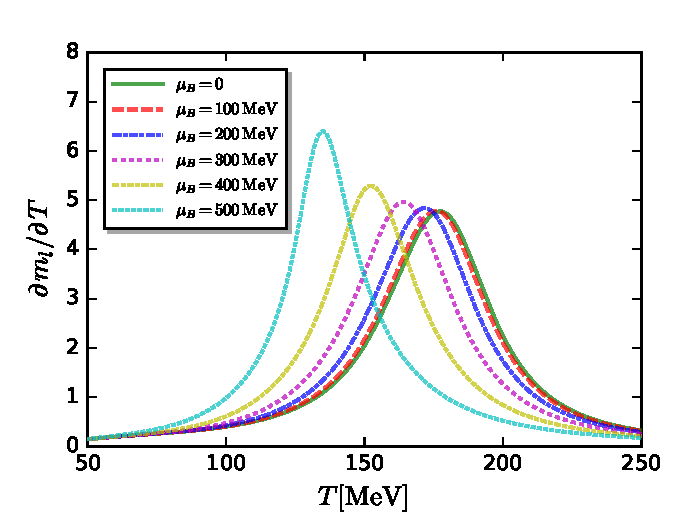
\includegraphics[width=0.45\textwidth]{dmfdT}
\caption{Constituent light quark mass (left panel) and its derivative to the temperature (right panel) as functions of the temperature with several values of baryon chemical potential.}
\label{fig:ml}
\end{figure*}
%%%%%%%%%%%%%%%%%%%%%%%%%%%%%
%

%
%%%%%%%%%%%%%%%%%%%%%%%%%%%%%
\begin{figure}[t]
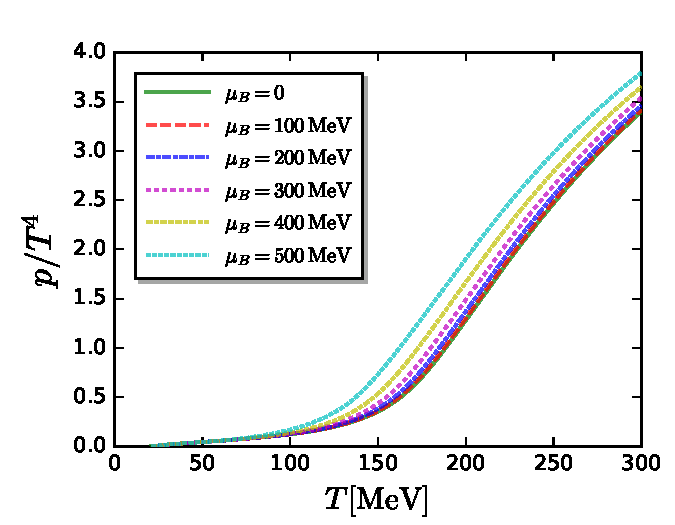
\includegraphics[width=0.45\textwidth]{poT4}
\caption{Pressure normalized by $T^4$ as a function of the temperature at baryon chemical potential $\mu_B=$ 0, 100, 200, 300, 400 and 500 MeV. These results are obtained in the 2+1 flavor LEFT.}
\label{fig:pressure}
\end{figure}
%%%%%%%%%%%%%%%%%%%%%%%%%%%%%
%

%
%%%%%%%%%%%%%%%%%%%%%%%%%%%%%
\begin{figure*}[t]
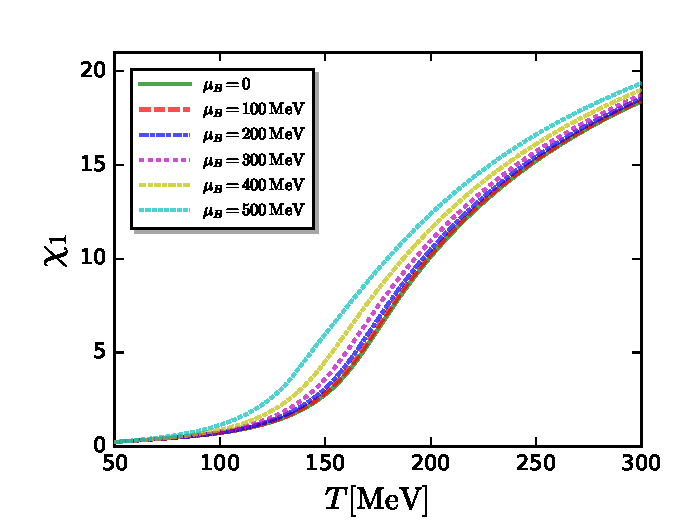
\includegraphics[width=0.45\textwidth]{chi1}\hspace{0.5cm}
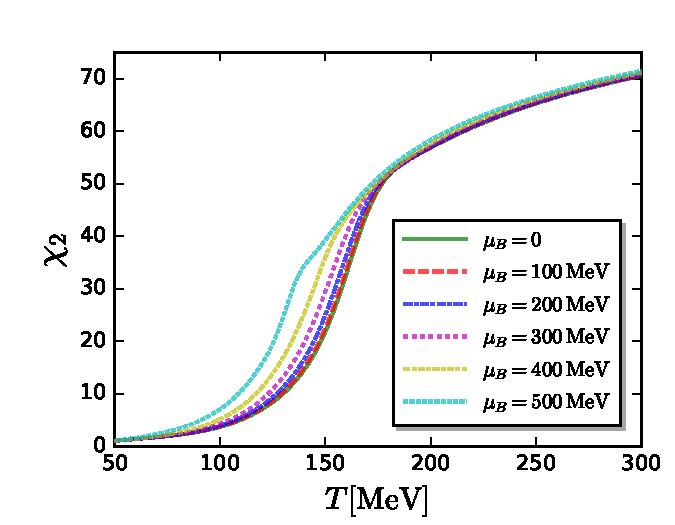
\includegraphics[width=0.45\textwidth]{chi2}
\caption{Dimensionless entropy (left panel) and heat capacity (right panel) normalized by appropriate powers of $T$, i.e., $\chi_1$ and $\chi_2$, as functions of the temperature with several values of baryon chemical potential.}
\label{fig:chi1-2}
\end{figure*}
%%%%%%%%%%%%%%%%%%%%%%%%%%%%%
%


%
%%%%%%%%%%%%%%%%%%%%%%%%%%%%%
\begin{figure*}[t]
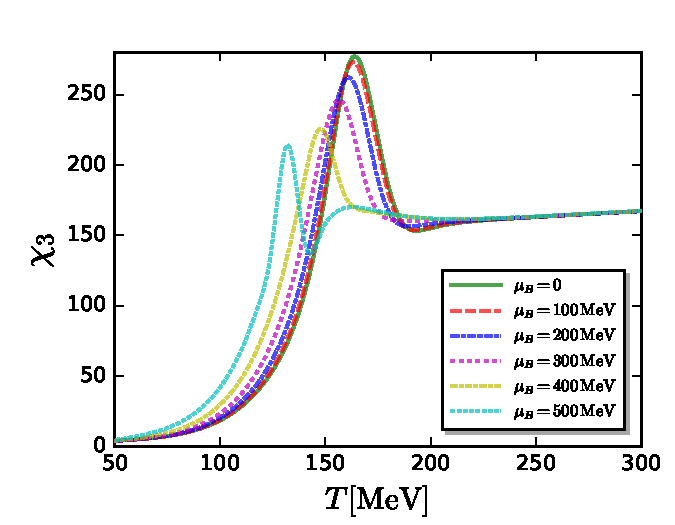
\includegraphics[width=0.45\textwidth]{chi3}\hspace{0.5cm}
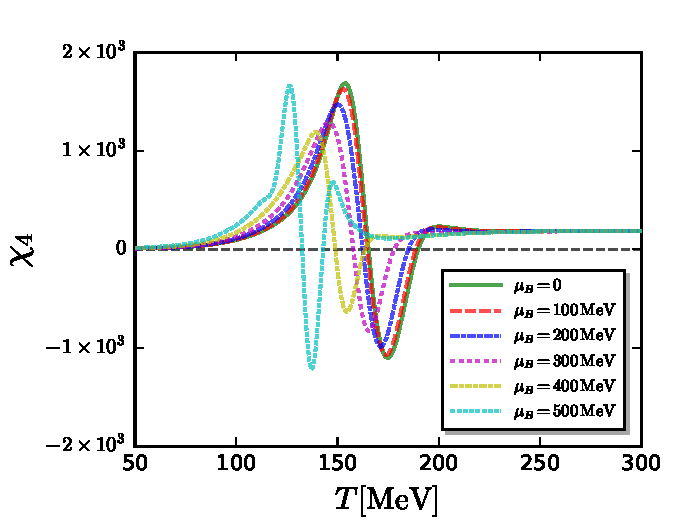
\includegraphics[width=0.45\textwidth]{chi4}
\caption{Skewness (left panel) and kurtosis (right panel) of the entropy fluctuations, i.e., $\chi_3$ and $\chi_4$, as functions of the temperature with several values of baryon chemical potential.}
\label{fig:chi3-4}
\end{figure*}
%%%%%%%%%%%%%%%%%%%%%%%%%%%%%
%


%
%%%%%%%%%%%%%%%%%%%%%%%%%%%%%
\begin{figure*}[t]
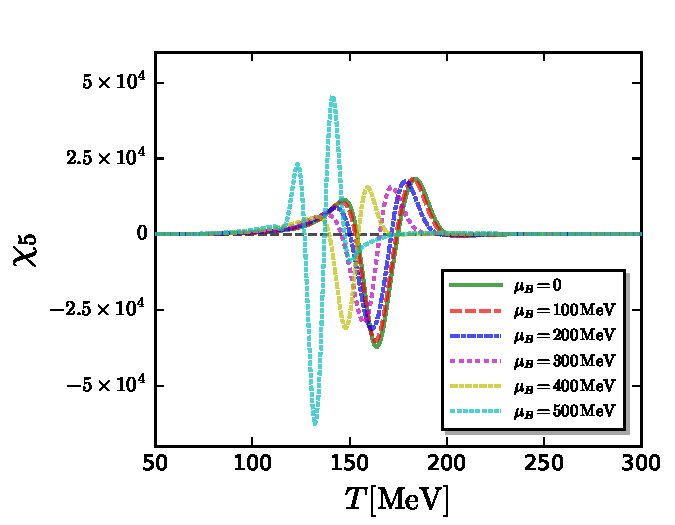
\includegraphics[width=0.45\textwidth]{chi5}\hspace{0.5cm}
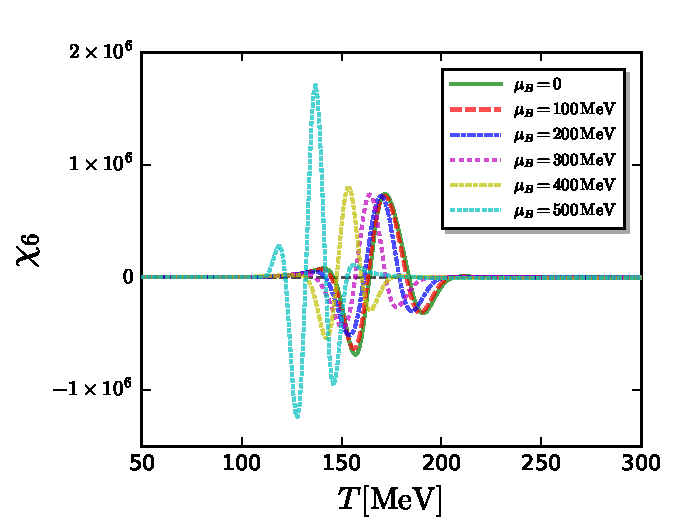
\includegraphics[width=0.45\textwidth]{chi6}
\caption{Fifth (left panel) and sixth (right panel) order fluctuations of the entropy, i.e., $\chi_5$ and $\chi_6$, as functions of the temperature with several values of baryon chemical potential.}
\label{fig:chi5-6}
\end{figure*}
%%%%%%%%%%%%%%%%%%%%%%%%%%%%%
%


The mesonic potential in \labelcref{eq:action}, i.e., the matter sector of the effective potential, reads
\begin{align}
    V_{\text{\tiny{matt}},k}(\phi)&=\tilde{V}_k(\rho_1,\rho_2)-c_A \xi-c_l\sigma_l-c_s\sigma_s\,, \label{eq:Vmatt}
\end{align}
with
\begin{align}
    \rho_1&=\text{tr}(\Sigma \cdot \Sigma^\dagger)\,, \label{eq:rho1}\\[2ex]
    \rho_2&=\text{tr}\Big(\Sigma \cdot \Sigma^\dagger-\frac{1}{3}\,\rho_1\,\mathbb{1}_{3\times 3}\Big)^2 \,,\label{eq:rho2}
\end{align}
where $\rho_1$ and $\rho_2$ are invariant under the transformations $\mathrm{SU}_{\mathrm{V}}(3)\times \mathrm{SU}_{\mathrm{A}}(3)\times \mathrm{U}_{\mathrm{V}}(1)\times \mathrm{U}_{\mathrm{A}}(1)$ in the flavor space. Here $\sigma_l$ and $\sigma_s$ indicate the scalar mesons of light and strange quarks, respectively. The relevant strength constants $c_l$ and $c_s$ result in explicit breaking of the chiral symmetry, as well as the breaking of the flavor symmetry from the three-flavor case to that of 2+1 flavors. The $\mathrm{U}_{\mathrm{A}}(1)$ symmetry is broken by the Kobayashi-Maskawa-'t Hooft determinant, viz.,
\begin{align}
    \xi=\det(\Sigma)+\det(\Sigma^\dagger)\,, \label{}
\end{align}
arising from quantum fluctuations, whose strength is controlled by the constant $c_A$.

The glue dynamics is encoded in the glue potential $V_{\mathrm{\tiny{glue}}}$ in \labelcref{eq:action}, also known as the Polyakov loop potential. The Polyakov loop is related to the temporal gluon background field $A_0$, that reads
\begin{align}
  L(\bm{x})=\frac{1}{N_c} \left\langle \Tr\, {\cal P}(\bm x)\right\rangle \,,\quad  \bar L (\bm{x})=\frac{1}{N_c} \langle
  \Tr\,{\cal P}^{\dagger}(\bm x)\rangle \,,\label{eq:Lloop}
\end{align}
with 
\begin{align}
  {\cal P}(\bm x)= \mathcal{P}\exp\Big(ig\int_0^{\beta}d\tau A_0(\bm{x},\tau)\Big)\,,\label{eq:Ploop}
\end{align}
where $\mathcal{P}$ on the right side denotes the path ordering, and $g$ is the strong coupling constant.

In this work, we employ the Haar glue potential \cite{Lo:2013hla, Wen:2018nkn}, 
\begin{align}
    V_{\text{\tiny{glue}}}(L, \bar L)=T^4 \,\bar V_{\text{glue-Haar}}\,,\label{eq:Vglue}
\end{align}
with
\begin{align}
    \bar V_{\text{glue-Haar}} &= -\frac{\bar a(T)}{2} \bar L L + \bar b(T)\ln M_H(L,\bar{L})+ \frac{\bar c(T)}{2} (L^3+\bar L^3) + \bar d(T) (\bar{L} L)^2\,,\label{eq:GluepHaar}
\end{align}
where the Haar measure reads
\begin{align}
    M_H (L, \bar{L})&= 1 -6 \bar{L}L + 4 (L^3+\bar{L}^3) - 3  (\bar{L}L)^2\,.
\end{align}
The temperature dependence of the coefficients $\bar a$, $\bar c$, $\bar d$ in \labelcref{eq:GluepHaar} is parameterized as
\begin{align}
    x(T) &= \frac{x_1 + x_2/(t+1) + x_3/(t+1)^2}{1 + x_4/(t+1) + x_5/(t+1)^2}\,,\quad x\in (\bar a, \bar c, \bar d)\,,\label{eq:xT}
\end{align}
and that of $\bar b$ as
\begin{align}
    \bar b(T) &=\bar b_1 (t+1)^{-\bar b_4}\left (1 -e^{\bar b_2/(t+1)^{\bar b_3}} \right)\,.\label{eq:bT}
\end{align}
Here $t$ in \labelcref{eq:xT,eq:bT} is the reduced temperature, that is
\begin{align}
    t&=\alpha (T-T_c^\mathrm{\tiny{glue}})/T_c^\mathrm{\tiny{glue}}\,,\label{}
\end{align}
where the parameters $T_c^\mathrm{\tiny{glue}}=250$ MeV and $\alpha=0.6$ are used throughout this work. The values of other parameters in \labelcref{eq:xT,eq:bT} can be found in \cite{Lo:2013hla, Wen:2018nkn}.

Moreover, using the same method in \cite{Fu:2023lcm}, we employ the dependence of the Yukawa coupling on the RG scale $k$ calculated from the first-principles QCD \cite{Fu:2019hdw}, as an input for the LEFT. Then the Yukawa coupling in the LEFT now reads
\begin{align}
    h_k&=h_0 \frac{h_{k}^{\mathrm{QCD}}}{h_{k=0}^{\mathrm{QCD}}}\,,\label{eq:hk}
\end{align}
where $h_{k}^{\mathrm{QCD}}$ is computed by using the fRG approach to the first-principles QCD in the vacuum \cite{Fu:2019hdw}, as shown in Fig.~\ref{fig:hQCD-k}. Here the parameter in the LEFT $h_0=12$ is determined by fitting the constituent light $u$ and $d$ quark mass $m_l=311$ MeV. Furthermore, we use the same values of parameters in the matter sector in \labelcref{eq:Vmatt} as those in \cite{Wen:2018nkn}.

In the left panel of Fig.~\ref{fig:ml}, we show the constituent masses for the $u$, $d$ light quarks calculated in the 2+1 flavor LEFT, depicted as functions of the temperature at several values of $\mu_B$. Their respective derivatives with respect to the temperature are shown in the right panel of Fig.~\ref{fig:ml}, from which one can determine the pseudo-critical temperature for the chiral crossover through the location of the peak. Figure~\ref{fig:pressure} displays the temperature dependence of pressure calculated in our 2+1 flavor LEFT-fRG framework for baryon chemical potential $\mu_B$ ranging from $\mu_B=0$ to 500 MeV, from which one can compute the temperature derivatives of pressure. The relevant results, from the first to sixth order derivatives, are presented in Figs.~\ref{fig:chi1-2} to~\ref{fig:chi5-6}, which stand for the entropy and its fluctuations of different orders.

%%%%%%%%%%%%%%%%%%%%%%%%%%%%%%%%%%%%
\subsection{Preliminary results of temperature fluctuations calculated in QCD within fRG}
\label{app:cn-QCD}

%
%%%%%%%%%%%%%%%%%%%%%%%%%%%%%
\begin{figure*}[t]
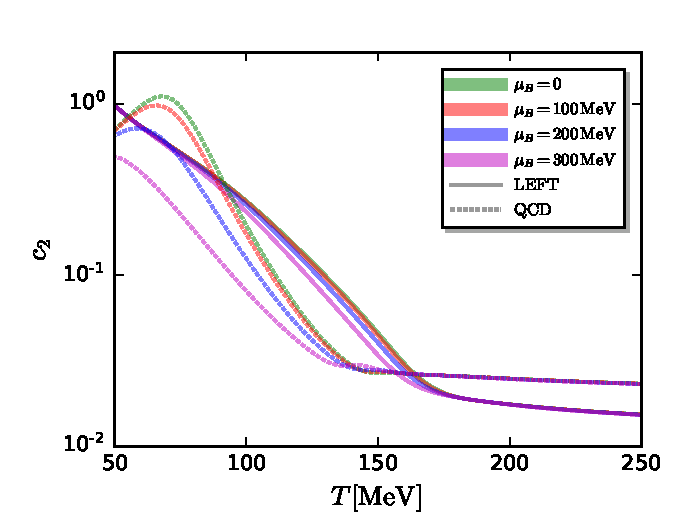
\includegraphics[width=0.45\textwidth]{c2-QCD}\hspace{0.5cm}
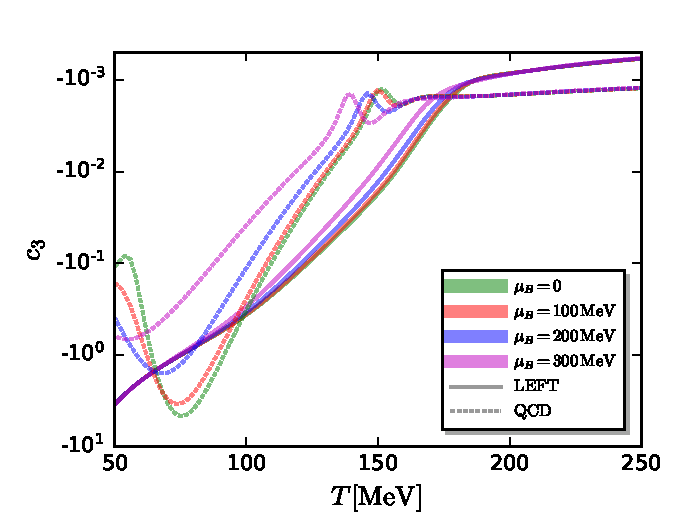
\includegraphics[width=0.45\textwidth]{c3-QCD}
\caption{Comparison between the LEFT and QCD computations for the second- and third-order fluctuations of temperature, i.e., $c_2$ (left panel) and $c_3$ (right panel), as functions of the temperature with several values of baryon chemical potential. The LEFT and QCD results are denoted by the solid and dashed lines, respectively.}
\label{fig:c1-2-QCD}
\end{figure*}
%%%%%%%%%%%%%%%%%%%%%%%%%%%%%
%

In addition, we also compare the temperature fluctuations obtained in the LEFT with the preliminary results obtained in QCD within the fRG, whose setup is detailed in \cite{Fu:2019hdw}. The relevant results are presented in Fig.~\ref{fig:c1-2-QCD}. One can see that although there are some differences, the variance and skewness of temperature fluctuations calculated from the LEFT and QCD are consistent with each other qualitatively. Note that the main conclusions obtained from the calculations in LEFT are corroborated by the QCD results, e.g., the skewness of temperature fluctuations is negative and the variance decreases significantly with the increase of temperature. 


%%%%%%%%%%%%%%%%%%%%%%%%%%%%%%%%%%%%
\subsection{Hyper-order fluctuations of temperature}
\label{app:hyper-order}

%
%%%%%%%%%%%%%%%%%%%%%%%%%%%%%
\begin{figure*}[t]
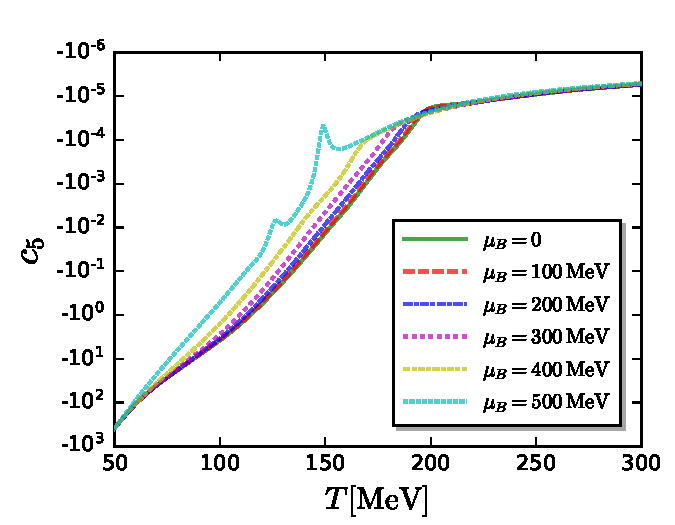
\includegraphics[width=0.45\textwidth]{c5}\hspace{0.5cm}
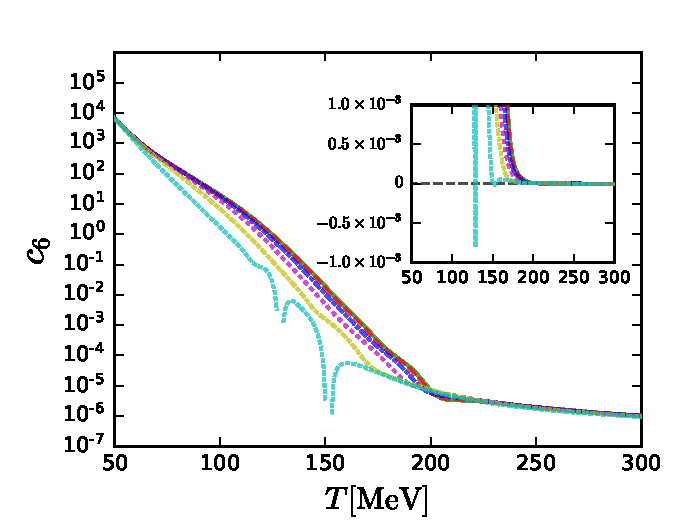
\includegraphics[width=0.45\textwidth]{c6}
\caption{Hyper-order fluctuations of temperature, $c_5$ (left panel) and $c_6$ (right panel), as functions of the temperature with several different values of baryon chemical potential. The inset on the right shows the plot by using the linear $y$-axis, where the zero-crossing for $c_6$ at high baryon chemical potential is clear.}
\label{fig:c5-6}
\end{figure*}
%%%%%%%%%%%%%%%%%%%%%%%%%%%%%
%

The fifth- and sixth-order fluctuations of temperature are given by
\begin{equation}\label{eq:c56}
\begin{split}
    c_5=&T^{11}\Bigg[-15\left(\frac{\partial^2 p}{\partial T^2}\right)^{-7}\left(\frac{\partial^3 p}{\partial T^3}\right)^3-\left(\frac{\partial^2 p}{\partial T^2}\right)^{-5}\frac{\partial^5 p}{\partial T^5}+10\left(\frac{\partial^2 p}{\partial T^2}\right)^{-6}\frac{\partial^3 p}{\partial T^3}\frac{\partial^4 p}{\partial T^4}\Bigg]\,\\[2ex]
     c_6=&T^{14}\Bigg[105\left(\frac{\partial^2 p}{\partial T^2}\right)^{-9}\left(\frac{\partial^3 p}{\partial T^3}\right)^4-105\left(\frac{\partial^2 p}{\partial T^2}\right)^{-8}\left(\frac{\partial^3 p}{\partial T^3}\right)^2\frac{\partial^4 p}{\partial T^4}+10\left(\frac{\partial^2 p}{\partial T^2}\right)^{-7}\left(\frac{\partial^4 p}{\partial T^4}\right)^2\\[2ex]
    &+15\left(\frac{\partial^2 p}{\partial T^2}\right)^{-7}\frac{\partial^3 p}{\partial T^3}\frac{\partial^5 p}{\partial T^5}-\left(\frac{\partial^2 p}{\partial T^2}\right)^{-6}\frac{\partial^6 p}{\partial T^6}\Bigg]\,.
\end{split} 
\end{equation}
The relevant numerical results are shown in Fig.~\ref{fig:c5-6}.


%%%%%%%%%%%%%%%%%%%%%%%%%%%%%%%%%%%%
\subsection{Ratios of temperature fluctuation cumulants}
\label{app:cn-ratios}

%
%%%%%%%%%%%%%%%%%%%%%%%%%%%%%
\begin{figure*}[t]
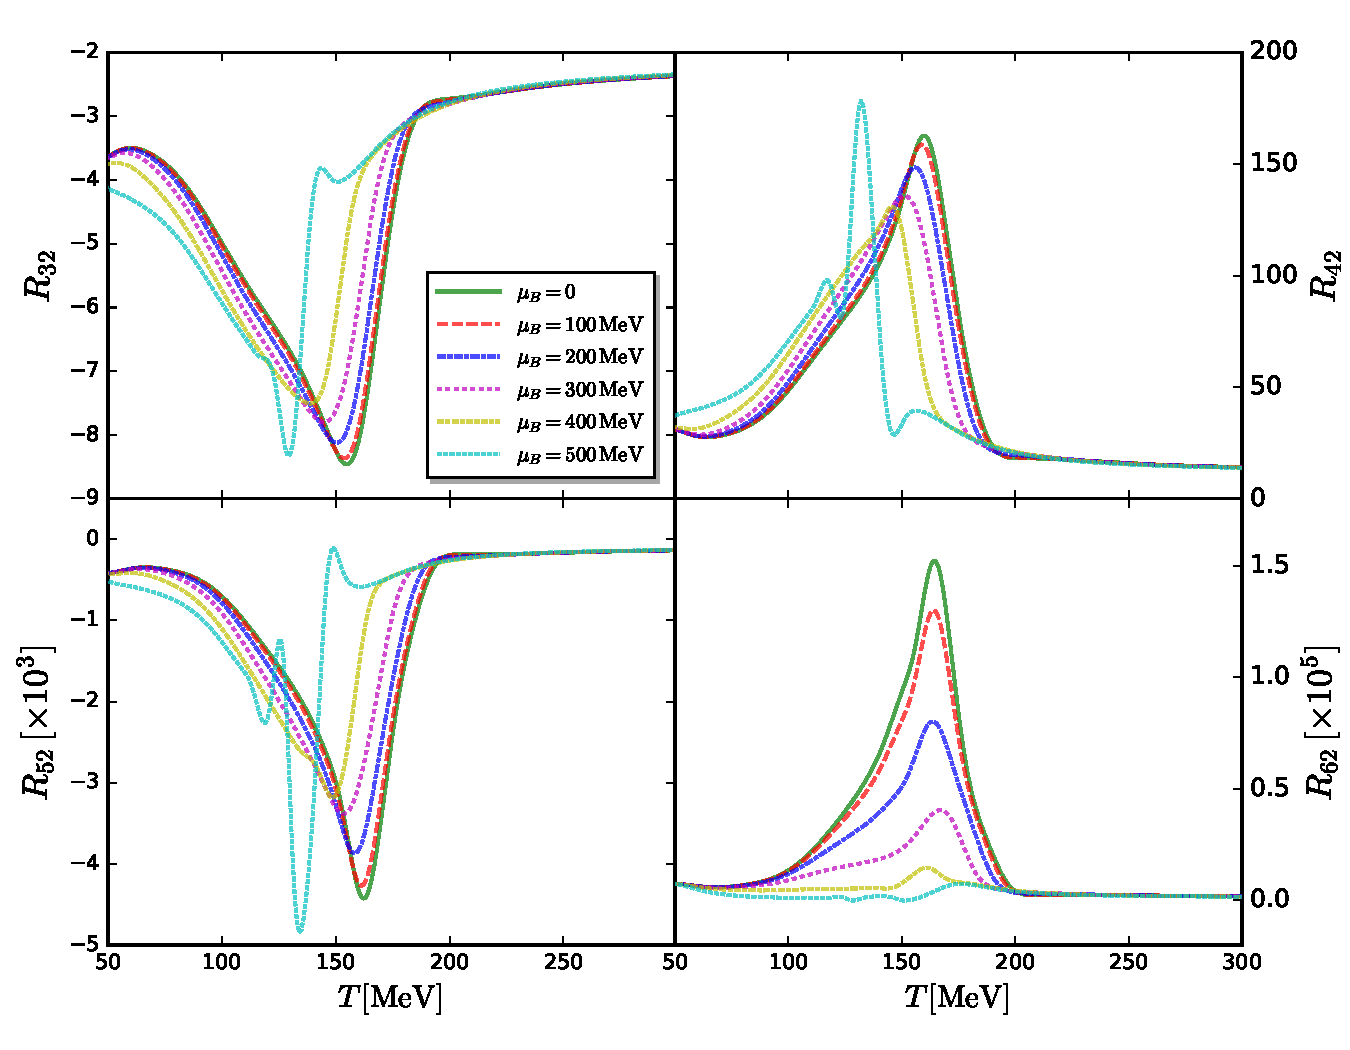
\includegraphics[width=0.8\textwidth]{Rmn}
\caption{Ratios between high-order temperature fluctuations and the variance, $R_{32}=c_3/c_2^2$, $R_{42}=c_4/c_2^3$, $R_{52}=c_5/c_2^4$, $R_{62}=c_6/c_2^5$, as functions of the temperature with several different values of baryon chemical potential.}
\label{fig:Rmn}
\end{figure*}
%%%%%%%%%%%%%%%%%%%%%%%%%%%%%
%

In relativistic heavy-ion collisions, the event-averaged mean transverse momentum $\langle p_{T} \rangle$ of charged particles exhibits an approximate linear dependence on the system temperature, $\langle p_{T} \rangle = a\,T$. The parameter $a$ represents the proportionality coefficient. In order to eliminate the influence from this coefficient that is not determined quite well, we instead analyze dimensionless ratios of temperature fluctuation cumulants: 
\begin{align}
    R_{32}=\frac{c_3}{c_2^2}\,, \quad R_{42}=\frac{c_4}{c_2^3}\,,\quad R_{52}=\frac{c_5}{c_2^4}\,,\quad R_{62}=\frac{c_6}{c_2^5}\,.\label{eq:R32R42}
\end{align}
where the powers of the variance in the denominators are chosen to balance the powers of $T$. The relevant ratios, presented in Fig.~\ref{fig:Rmn}, reveal that the cumulant ratios develop an increasingly rich nonmonotonic structure while exhibiting systematically reduced amplitudes with the increase of $\mu_B$, reflecting competing effects where enhanced critical fluctuations near the sharpened phase boundary emerge concurrently with the overall suppression of the magnitude of temperature fluctuation. 

%%%%%%%%%%%%%%%%%%%%%%%%%%%%%%%%%%%%
\subsection{Relation between the temperature $T$ and the mean transverse momentum $\langle p_{T} \rangle$}
\label{app:T-pT-relation}

Considering a free relativistic gas in thermal equilibrium at temperature $T$ with Boltzmann statistics, where the mass of particle, e.g., the pion $m_\pi\sim 150 $ MeV, is negligible in comparison to the typical value of the transverse momentum $p_T \sim 1$ GeV, the particle number reads
\begin{align}
    N=(2s+1)V\int \frac{d^3 p}{(2\pi)^3}e^{-p/T}\,, \label{eq:N}
\end{align}
where $s$ denotes the spin of the particle and $V$ the volume of system. One readily finds for the mean transverse momentum of particles
\begin{align}
    \langle p_{T} \rangle=\frac{1}{N}(2s+1)V\int \frac{d^3 p}{(2\pi)^3}\,p_{T}\,e^{-p/T}\,, \label{eq:pt}
\end{align}
where the momentum and the transverse momentum is related through
\begin{align}
    p=\sqrt{p_{T}^2+p_z^2}\,, \label{}
\end{align}
with the longitudinal momentum $p_z$. Combining Eqs.~\labelcref{eq:N} and \labelcref{eq:pt} we have
\begin{align}
    \langle p_{T} \rangle=\frac{\int \frac{d^3 p}{(2\pi)^3}\,p_{T}\,e^{-p/T}}{\int \frac{d^3 p}{(2\pi)^3}\,e^{-p/T}}\,. \label{eq:pt2}
\end{align}
From the dimensional analysis in Eqs.~\labelcref{eq:pt2}, one immediately arrives at
\begin{align}
    \langle p_{T} \rangle=a\, T\,, \label{eq:pt-T}
\end{align}
that is, $\langle p_{T} \rangle$ is linearly proportional to the temperature, with the proportionality coefficient $a$. Note that this is different from the non-relativistic case, where it is easy to find that $\langle p_{T} \rangle \sim T^{1/2}$. In order to determine the coefficient $a$ in Eq.~\labelcref{eq:pt-T}, one has to compute the expression in Eq.~\labelcref{eq:pt2}. The integral in the numerator in Eq.~\labelcref{eq:pt2} cannot be computed analytically, but one can expand the momentum in the exponent in powers of $p_z/p_{T}$, i.e.,
\begin{align}
    p&=p_{T}\Big(1+\frac{p_z^2}{p_{T}^2}\Big)^{1/2} \nonumber\\[2ex]
    &=p_{T}+\frac{1}{2}\frac{p_z^2}{p_{T}}+\cdots\,.\label{eq:pexpan}
\end{align}
Expanding Eq.~\labelcref{eq:pexpan} to the second order, and substituting into Eq.~\labelcref{eq:pt2}, one finds
\begin{align}
    \langle p_{T} \rangle \approx \frac{15}{16\sqrt{2}}\pi T \approx 2.08 \,T\,. \label{}
\end{align}
Note that this value is close to the exact value
\begin{align}
    a=2.356\,, \label{}
\end{align}
obtained by directly computing Eq.~\labelcref{eq:pt2} numerically.


\bibliography{ref-lib}% Produces the bibliography via BibTeX.


%\vfill 

\end{document} 